\section{Greedy-Algorithmen}
\begin{sectionbox}
\subsection{Eigenschaften}
Ein rekursiv lösbares Optimierungsproblem kann mit einem \textbf{gierigen (greedy) Algorithmus} gelöst werden, wenn es die folgende Eigenschaften hat:
\begin{itemize}
    \item Das Problem hat \textbf{optimale Substruktur}: die Lösung eines Problems ergibt sich durch Kombination optimaler Teillösungen.
    \item Es gilt die \textbf{greedy choice property}: Die Lösung eines Problems kann konstruiert werden, indem ein lokales Kriterium herangezogen wird, welches nicht von der Lösung der Teilprobleme abhängt.    
\end{itemize}
\end{sectionbox}
\vspace{-4pt}
\begin{sectionbox}
\subsection{Huffman-Code} 
Betrachten Präfixcodes: kein Codewort kann mit einem anderen Codewort beginnen.\par
Präfixcodes können im Vergleich mit allen Codes die optimale Datenkompression erreichen.\par\smallskip
\begin{center}
    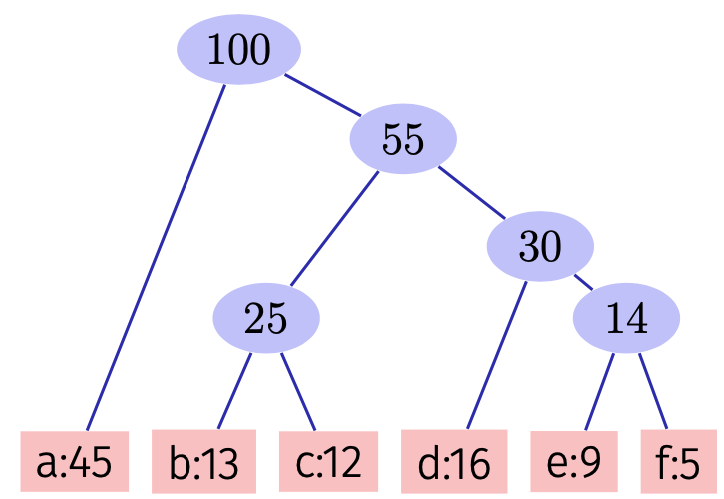
\includegraphics[width=0.35 \columnwidth]{img/HuffmanImg.png}
\end{center}\par\smallskip

\textbf{Huffman(C)}
\begin{center}
    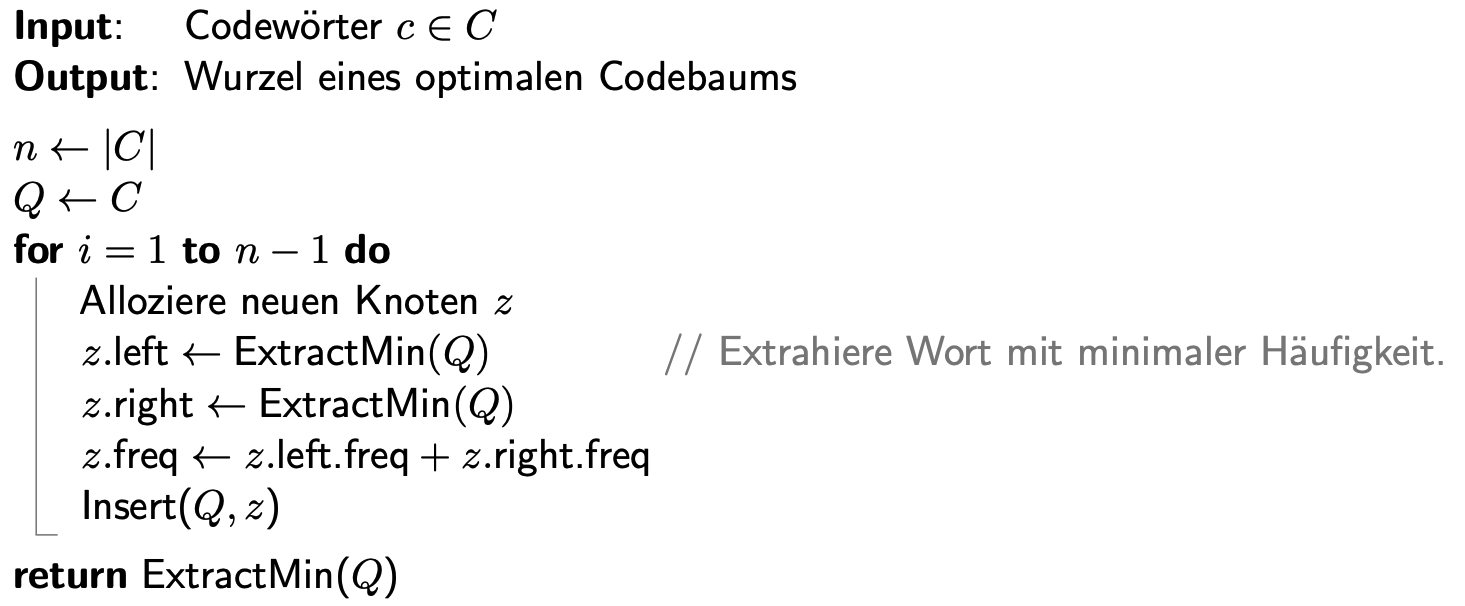
\includegraphics[width= \columnwidth]{img/HuffmanAlgo.png}
\end{center}\par\smallskip

\textbf{Analyse}: Heap bauen in $\mathcal{O}(n)$. Extract-Min in $\mathcal{O}(\log (n))$ für $n$ Elemente. Somit Laufzeit $\mathcal{O}b(n \log(n))$.
\end{sectionbox}

